\documentclass[12pt, a4paper, oneside]{article}
\usepackage{seephy}
\title{\textbf{Computational Physics(A) \\Assignment 2}}
\author{Chon Hei Lo\thanks{Email: see.looooo@stu.pku.edu.cn; StudentID: 2000012508} (罗俊熙) \\ School of Physics, Peking University}
\date{\today}
\linespread{1.5}

\newcounter{problemname}
\begin{document}

\maketitle

\begin{center}
\textit{注1: 此作业的解答如无说明,统一使用爱因斯坦求和约定。}
\textit{P.S.: 这次作业为甚么题目没有标题和分值QQ,强迫症受不了QQ}
\end{center}
\section{Problems \& Solutions}
% ==============================Problem 1==================================
\subsection{解方程组}
编写高斯消元法和 Cholesky 方法的代码,并求解如下线性方程组:
\begin{align*}
    \left\{
        \begin{array}{ccc}
        0.05x_1+0.07x_2+0.06x_3+0.05x_4 &= 0.23 \\
        0.07x_1+0.10x_2+0.08x_3+0.07x_4 &= 0.32 \\
        0.06x_1+0.08x_2+0.10x_3+0.09x_4 &= 0.33 \\
        0.05x_1+0.07x_2+0.09x_3+0.10x_4 &= 0.31
        \end{array}
    \right.
\end{align*}


% ==============================Solution 1==================================
\textbf{Solution:}此题基本和上一次作业一样,所使用的代码片段如下:
\begin{figure}
    \centering
    
\includegraphics[width=0.7\textwidth]{fig1.png}
    \caption{高斯消元法的代码片段}
\end{figure}

\begin{figure}
    \centering
    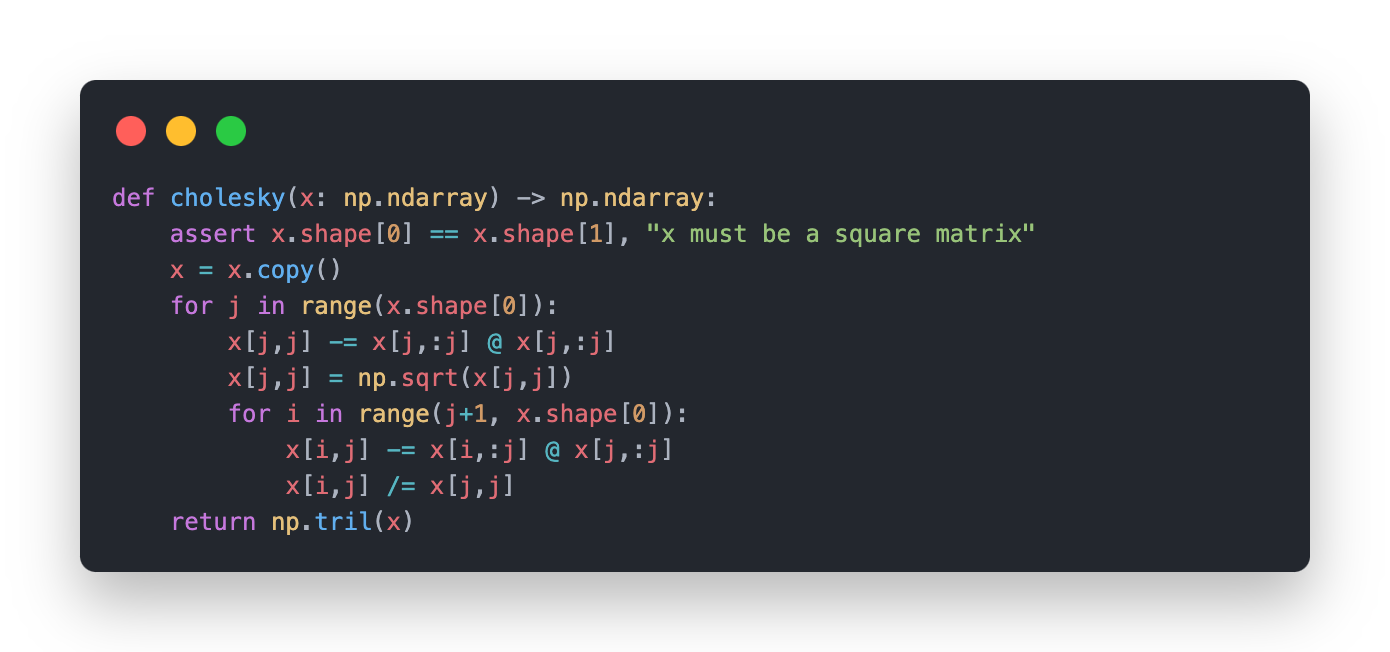
\includegraphics[width=0.7\textwidth]{fig2.png}
    \caption{Cholesky 方法的代码片段}
\end{figure}

两者结果一样,均为$x=\ab[1,1,1,1]^T$
\clearpage
% ==============================Problem 2==================================
\subsection{样条函数插值}
对$f(x)=\cos(x^2)$,采用三次样条插值。分别考虑如下两种边界条件:
\begin{enumerate}[(a)]
    \item $x_0=0$ 和 $x_2=0.9$ 端点处的二次导数值为$0$;
    \item 利用$f(x)$得到$x_0=0$和$x_2=0.9$端点处的一次导数值。
\end{enumerate}

% ==============================Solution 2==================================    
\textbf{Solution:}参考代码\file{2-2.py}和\file{seelib.spline.py},代码这里就不重复贴上了,结果如下
\begin{figure}[h]
    \centering
    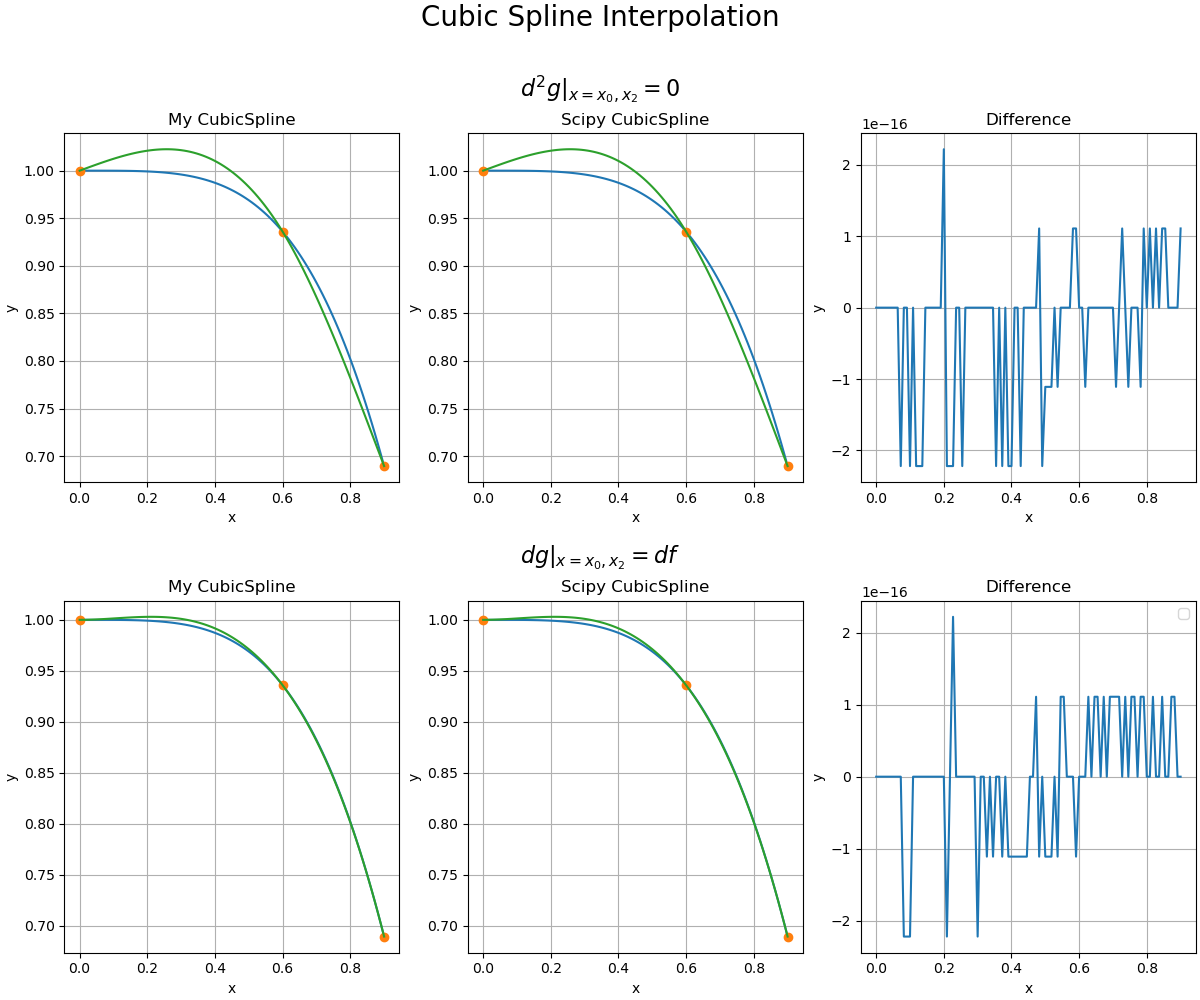
\includegraphics[width=1.0\textwidth]{fig3.png}
    \caption{两种边界条件下的样条函数插值}

\end{figure}

\clearpage
% ==============================Problem 3==================================
\subsection{Runge 效应}
考虑 Runge 函数 $f(x)=\frac{1}{1+25x^2}$ 在区间$[-1,1]$上的行为。本题中将分别利用等间距的多项式内插、Chebyshev 内插以及三次样条函数来近似$f(x)$的数值。
\begin{enumerate}[(a)]
    \item 考虑$[-1,1]$上的 21 个均匀分布的节点(包括端点,相隔 $0.1$ 一个点)的 $20$ 阶多项式$P_{20}(x)$之内插(你可以利用各种方法,例如拉格朗日内插、牛顿内插或者 Neville 方法)。给出一个表分别列出$x$,$f(x)$,$P_{20}(x)$以及两者差的绝对值。为了看出两者的区别请在这 21 个点分成的每个小段的中点也取一个数据点并一起列出 (因此共有 41 个点),同时画图显示之。
    \item 现在选取$n=20$并将上问中均匀分布的节点换为标准的 Chebyshev 节点:
        $$x_k= \cos\ab(\frac{k+1/2}{20}\pi),\quad k=0,1,\cdots,19$$
        然后构造$f(x)$在$[-1,1]$上的近似式,
        $$f(x)\approx C(x)\equiv -\frac{c_0}{2}+\sum_{k=0}^{20}c_kT_k(x)$$
        其中在各个 Chebyshev 的节点处我们要求它严格等于$f(x)$ 。同样列出上问的表并画图,与上问结果比较。

    \item 仍然考虑第一问中均匀分布的 $21$ 个节点的内插。但这次利用 $21$ 点的三次样条函数。
    重复上面的列表、画图并比较。
\end{enumerate}

% ==============================Solution 3==================================
\textbf{Solution:}参考代码\file{2-3.py},插值结果如\autoref{fig:4},它们值的差异在\autoref{tab:1}所示,可以看见在两边出现了巨大的差异。


\begin{longtable}{|c|c||c|c||c|c||c|c|}
    \caption{Runge 函数的插值结果\label{tab:1}}\\
    \hline
    $x$ & $f(x)$ & $P_{20}(x)$ & $\ab\vert P_{20}(x) - f(x)\vert$ & $T(x)$ & $\ab\vert T(x) - f(x) \vert$ & $S(x)$ & $\ab\vert S(x) - f(x) \vert$ \\
    \hline
    \endhead
    \hline
    \endfoot
    -1.00 & 0.04 & 0.04 & 0.00 & 0.04 & 0.01 & 0.04 & 0.00 \\
    -0.95 & 0.04 & -39.95 & 39.99 & 0.05 & 0.01 & 0.04 & 0.00 \\
    -0.90 & 0.05 & 0.05 & 0.00 & 0.04 & 0.01 & 0.05 & 0.00 \\
    -0.85 & 0.05 & 3.45 & 3.40 & 0.06 & 0.00 & 0.05 & 0.00 \\
    -0.80 & 0.06 & 0.06 & 0.00 & 0.06 & 0.00 & 0.06 & 0.00 \\
    -0.75 & 0.07 & -0.45 & 0.51 & 0.06 & 0.01 & 0.07 & 0.00 \\
    -0.70 & 0.08 & 0.08 & 0.00 & 0.07 & 0.00 & 0.08 & 0.00 \\
    -0.65 & 0.09 & 0.20 & 0.12 & 0.09 & 0.01 & 0.09 & 0.00 \\
    -0.60 & 0.10 & 0.10 & 0.00 & 0.11 & 0.01 & 0.10 & 0.00 \\
    -0.55 & 0.12 & 0.08 & 0.04 & 0.11 & 0.00 & 0.12 & 0.00 \\
    -0.50 & 0.14 & 0.14 & 0.00 & 0.13 & 0.01 & 0.14 & 0.00 \\
    -0.45 & 0.16 & 0.18 & 0.01 & 0.16 & 0.00 & 0.16 & 0.00 \\
    -0.40 & 0.20 & 0.20 & 0.00 & 0.21 & 0.01 & 0.20 & 0.00 \\
    -0.35 & 0.25 & 0.24 & 0.01 & 0.26 & 0.01 & 0.25 & 0.00 \\
    -0.30 & 0.31 & 0.31 & 0.00 & 0.31 & 0.00 & 0.31 & 0.00 \\
    -0.25 & 0.39 & 0.40 & 0.00 & 0.38 & 0.01 & 0.39 & 0.00 \\
    -0.20 & 0.50 & 0.50 & 0.00 & 0.49 & 0.01 & 0.50 & 0.00 \\
    -0.15 & 0.64 & 0.64 & 0.00 & 0.64 & 0.00 & 0.64 & 0.00 \\
    -0.10 & 0.80 & 0.80 & 0.00 & 0.81 & 0.01 & 0.80 & 0.00 \\
    -0.05 & 0.94 & 0.94 & 0.00 & 0.95 & 0.01 & 0.94 & 0.00 \\
    0.00 & 1.00 & 1.00 & 0.00 & 1.00 & 0.00 & 1.00 & 0.00 \\
    0.05 & 0.94 & 0.94 & 0.00 & 0.95 & 0.01 & 0.94 & 0.00 \\
    0.10 & 0.80 & 0.80 & 0.00 & 0.81 & 0.01 & 0.80 & 0.00 \\
    0.15 & 0.64 & 0.64 & 0.00 & 0.64 & 0.00 & 0.64 & 0.00 \\
    0.20 & 0.50 & 0.50 & 0.00 & 0.49 & 0.01 & 0.50 & 0.00 \\
    0.25 & 0.39 & 0.40 & 0.00 & 0.38 & 0.01 & 0.39 & 0.00 \\
    0.30 & 0.31 & 0.31 & 0.00 & 0.31 & 0.00 & 0.31 & 0.00 \\
    0.35 & 0.25 & 0.24 & 0.01 & 0.26 & 0.01 & 0.25 & 0.00 \\
    0.40 & 0.20 & 0.20 & 0.00 & 0.21 & 0.01 & 0.20 & 0.00 \\
    0.45 & 0.16 & 0.18 & 0.01 & 0.16 & 0.00 & 0.16 & 0.00 \\
    0.50 & 0.14 & 0.14 & 0.00 & 0.13 & 0.01 & 0.14 & 0.00 \\
    0.55 & 0.12 & 0.08 & 0.04 & 0.11 & 0.00 & 0.12 & 0.00 \\
    0.60 & 0.10 & 0.10 & 0.00 & 0.11 & 0.01 & 0.10 & 0.00 \\
    0.65 & 0.09 & 0.20 & 0.12 & 0.09 & 0.01 & 0.09 & 0.00 \\
    0.70 & 0.08 & 0.08 & 0.00 & 0.07 & 0.00 & 0.08 & 0.00 \\
    0.75 & 0.07 & -0.45 & 0.51 & 0.06 & 0.01 & 0.07 & 0.00 \\
    0.80 & 0.06 & 0.06 & 0.00 & 0.06 & 0.00 & 0.06 & 0.00 \\
    0.85 & 0.05 & 3.45 & 3.40 & 0.06 & 0.00 & 0.05 & 0.00 \\
    0.90 & 0.05 & 0.05 & 0.00 & 0.04 & 0.01 & 0.05 & 0.00 \\
    0.95 & 0.04 & -39.95 & 39.99 & 0.05 & 0.01 & 0.04 & 0.00 \\
    1.00 & 0.04 & 0.04 & 0.00 & 0.04 & 0.01 & 0.04 & 0.00 \\

\end{longtable}

\begin{figure}[H]
    \centering
    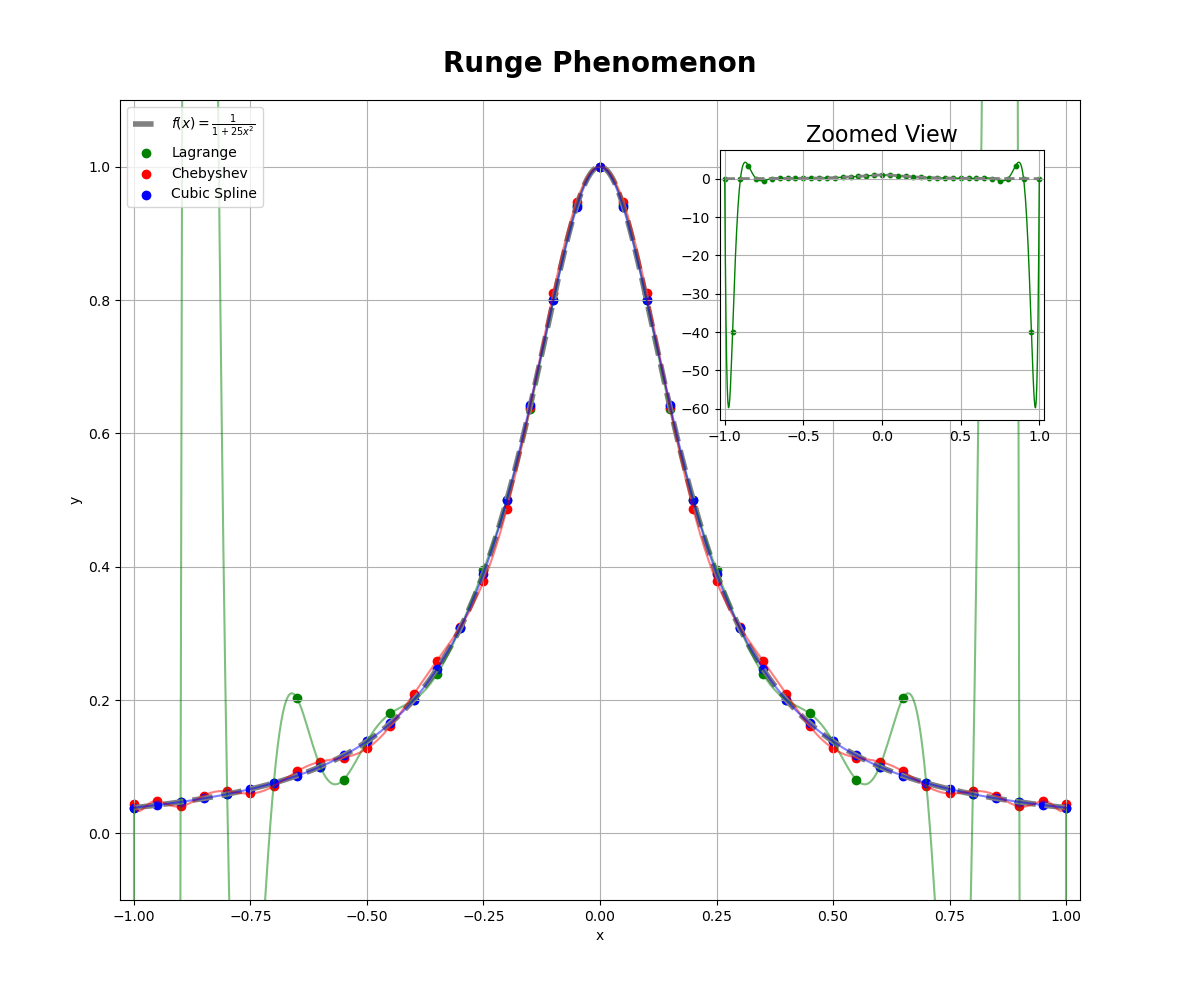
\includegraphics[width=1.0\textwidth]{fig4.png}
    \caption{Runge 函数的插值结果}

\end{figure}

% ==============================Problem 4==================================
\subsection{样条函数在计算机绘图中的运用}
本题中我们考虑 Cubic spline 在计算机绘图中的广泛运用。我们将尝试用三次样条函数平滑地连接若干个二维空间中已知的点。考虑二维空间的一
系列点$(x_i,y_i),\quad i=0,1\cdots n$。我们现在希望按照顺序(由 $0$ 到 $n$)将它们平滑地连接起来。一个方便的办法是引入一个连
续参数$t\in\ab[0,n]$,取节点为$t_i=0,1,\cdots,n$ ,然后分别建立两个样条函数:$S_\Delta\ab(X;t)$和$S_\Delta\ab(Y;t)$它们分别满足
\begin{align*}
    S_\Delta\ab(X;t_i)&=x_i\\
    S_\Delta\ab(Y;t_i)&=y_i
\end{align*}

这两个样条函数可以看作是$\ab(x(t),y(t))$的内插近似。因此绘制参数曲线$\ab(x(t),y(t))$的问题
就化为求出两个样条函数并将它们画出的问题。我们考虑的函数是着名的心形线(cardioid)。
它的极坐标方程是:
$$r(\phi)=2a\ab(1-\cos\phi)$$
为了方便起见我们取了$2a=1$。(请利用上一题中关于样条函数内插的相应代码来处理本题)
\begin{enumerate}[(a)]
    \item 选取$\phi=t\pi/4,\quad t=0,1,\cdots,8$这九个点,结出$x_t=r(\phi)\cos\phi$和$y_t=r(\phi)\cos\phi$的数值。将这些数值作为精确的数值列在一个表里。
    \item 给出过这 8 个点的两个三次样条函数$S_\Delta\ab(X;t)$和$S_\Delta\ab(Y;t)$。
    \item 画出参数形式的曲线$\ab(x_t, y_t)=\ab(S_\Delta\ab(X;t),S_\Delta\ab(Y;t))$同时画出它所内插的严格的曲
    线进行比较,请标出相应的节点。
    \item 简要说明为什么这个算法可以平滑地连接所有的点 (这实际上是很多画图软件中spline 曲线所采用的算法)。
\end{enumerate}

% ==============================Solution 4==================================
\textbf{Solution:}参考代码\file{2-4.py},可以给出这九个点的数据,如下表:
\begin{table}[H]
    \centering
    \caption{心形线的数据}
    \label{tab:2}
    \begin{tabular}{|c|c|c|c|c|c|c|c|c|c|}
        \hline
        $t$ & 0 & 1 & 2 & 3 & 4 & 5 & 6 & 7 & 8\\
        \hline
        $x_t$ & 0.00 & 0.21 & 0.00 & -1.21 & -2.00 & -1.21 & 0.00 & 0.21 & 0.00 \\
        \hline
        $y_t$ & 0.00 & 0.21 & 1.00 & 1.21 & 0.00 & -1.21 & -1.00 & -0.21 & 0.00 \\
        \hline
    \end{tabular}
\end{table}
分别画出$x$和$y$的三次样条函数,如\autoref{fig:5}所示。
\begin{figure}[H]
    \centering
    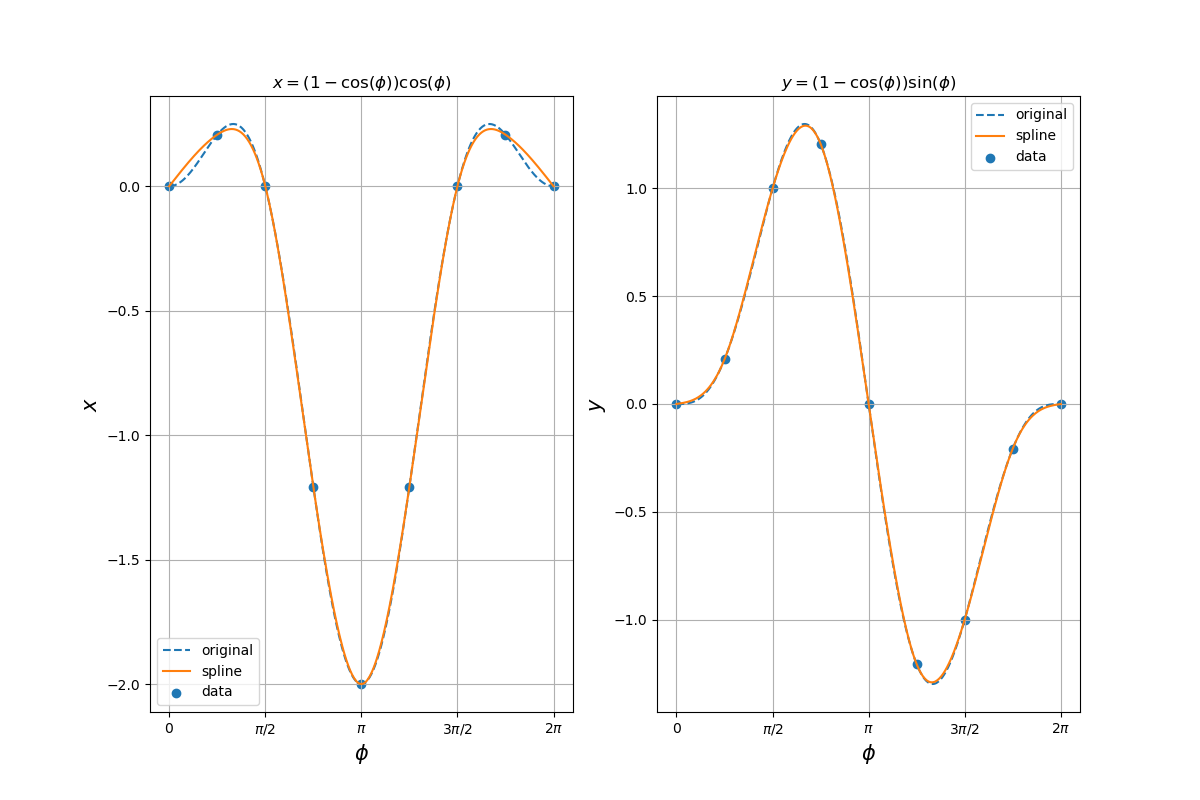
\includegraphics[width=1.0\textwidth]{fig6.png}
    \caption{两个参数方程分别的插值结果}
    \label{fig:5}
\end{figure}
通过三次样条函数,可以得到如下的结果:
\begin{figure}[H]
    \centering
    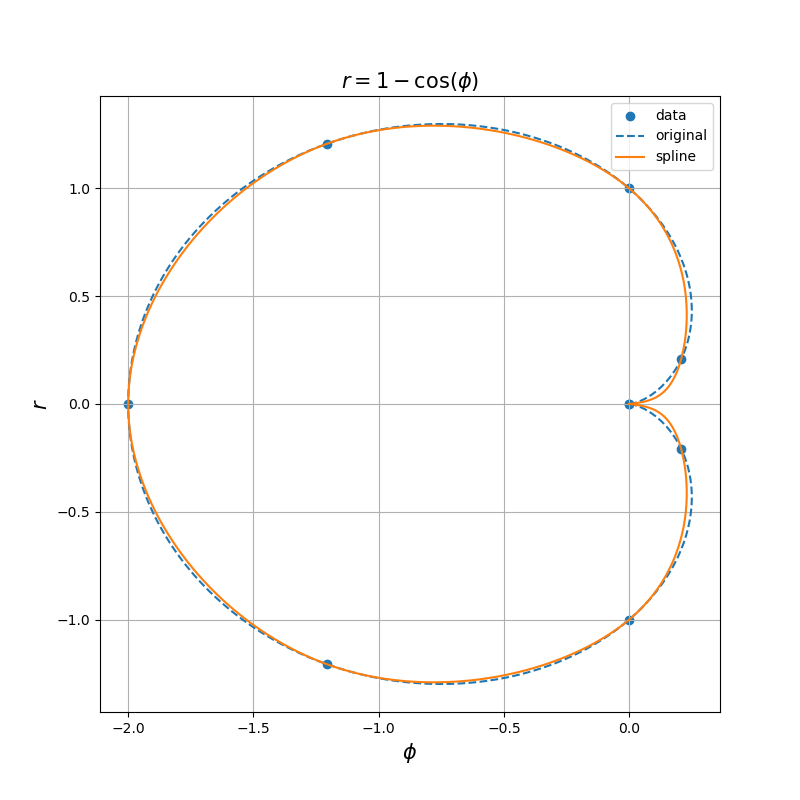
\includegraphics[width=1.0\textwidth]{fig5.png}
    \caption{心形线的插值结果}
\end{figure}
因为样条函数是连续可导的,因此$f\ab(x(t),y(t))$也是可导的,因此可以平滑地连接所有的点。

% ==============================Problem 5==================================
\subsection{对称矩阵特征值问题}
考虑一个对称矩阵
$$H=\begin{pmatrix}
    2 & -1 & 0 \\
    -1 & 2 & -1 \\
    0 & -1 & 1
\end{pmatrix}$$
\begin{enumerate}[(a)]
    \item 通过消元法求出三角矩阵 $L$ 和对角矩阵 $D$,使$H=LDL^T$。
    \item 可以将矩阵$H$ 的一个角元$H_{33} = 1$ 替换为$q$ ,使矩阵$H$ 为半正定,求出最小的$q$。
    \item 当$H_{33} = 2$时,求解其本征值。进而求出扩展到$4\times 4$矩阵$H^\prime$时的本征值。
    $$H^\prime=\begin{pmatrix}
        2 & -1 & 0 & 0 \\
        -1 & 2 & -1 & 0 \\
        0 & -1 & 2 & -1 \\
        0 & 0 & -1 & 2
    \end{pmatrix}$$
\end{enumerate}

% ==============================Solution 5==================================
\textbf{Solution:}
\begin{enumerate}[(a)]
    \item 使用高斯消元法进行消元,可以得到:
    \begin{NiceMatrixBlock}[auto-columns-width]
        \setlength{\extrarowheight}{1mm}
        \begin{align*}
            \begin{bNiceMatrix}[margin]
                \Block{3-3}<\Large>{H}& & \\
                & \hspace*{0.5cm} & \\
                & & \\ 
                \hline
                1 & 0 & 0 \\
                0 & 1 & 0 \\
                0 & 0 & 1
            \end{bNiceMatrix}
            &\Rightarrow 
            \begin{bNiceMatrix}[margin]
                2& 0& 0\\
                0& \frac32& -1\\
                0& -1& 1\\ 
                \hline
                1 & \frac12 & 0 \\
                0 & 1 & 0 \\
                0 & 0 & 1
            \end{bNiceMatrix}\\
            &\Rightarrow
            \begin{bNiceMatrix}[margin]
                2& 0& 0\\
                0& \frac32& 0\\
                0& 0& \frac13\\ 
                \hline
                1 & \frac12 & \frac13 \\
                0 & 1 & \frac23 \\
                0 & 0 & 1
            \end{bNiceMatrix}
        \end{align*}
    \end{NiceMatrixBlock}
    记$U^{-1}=\begin{bNiceMatrix}[margin]
        1 & \frac12 & \frac13 \\
        0 & 1 & \frac23 \\
        0 & 0 & 1
    \end{bNiceMatrix}$
    和$D=\begin{bNiceMatrix}[margin]
        2 &         &  \\
          & \frac32 &  \\
          &         & \frac13
    \end{bNiceMatrix}$,求解$U$:
    \begin{NiceMatrixBlock}[auto-columns-width]
        \setlength{\extrarowheight}{1mm}
        \begin{align*}
            &\begin{bNiceArray}{ccc|ccc}[margin]
                \Block{3-3}<\Large>{U^{-1}} & & & \Block{3-3}<\Large>{I} & & \\
                & \hspace*{0.5cm} & & & & \\
                & & & & &
            \end{bNiceArray}\\
            =&
            \begin{bNiceArray}{ccc|ccc}[margin]
                1& \frac12& \frac13 & 1& 0& 0\\
                 & 1      & \frac23 & 0& 1& 0\\
                 &        &       1 & 0& 0& 1
            \end{bNiceArray}\\
            \Rightarrow&
            \begin{bNiceArray}{ccc|ccc}[margin]
                1& \frac12& 0 & 1& 0& -\frac13\\
                 & 1      & 0 & 0& 1& -\frac23\\
                 &        & 1 & 0& 0& 1
            \end{bNiceArray}\\
            \Rightarrow&
            \begin{bNiceArray}{ccc|ccc}[margin]
                1& 0 & 0 & 1& -\frac12& 0\\
                 & 1 & 0 & 0& 1& -\frac23\\
                 &   & 1 & 0& 0& 1
            \end{bNiceArray}\\
        \end{align*}
    \end{NiceMatrixBlock}
    得到$L=\begin{bNiceMatrix}[margin]
        1 &       &  \\
         -\frac12 & 1 &  \\
          &    -\frac23     & 1
    \end{bNiceMatrix}$。
    容易验证$H=LDL^T$(或者使用\file{2-5.py})进行检验。
    \item 在进行变换的过程中,我们轻松地发现了角元$H_{33}=q$的改变对$L$不会影响,那么$D_{33}=q-\frac{2}{3}$,若要求$H$半正定,那么$D_{33}\ge0$,可知$q\ge \frac{2}{3}$。
    \item 直接展开其特征多项式:
        $$\ab|\lambda I - H| = (\lambda - 2)^4 - 3(\lambda -2)^2 + 1$$
        得到$(\lambda-2)^2=\frac{3\pm\sqrt{5}}{2}$,故特征值有4个,分别为:
        \begin{align*}
            \lambda_1&=2+\sqrt{\frac{3+\sqrt{5}}{2}}\\
            \lambda_2&=2-\sqrt{\frac{3+\sqrt{5}}{2}}\\
            \lambda_3&=2+\sqrt{\frac{3-\sqrt{5}}{2}}\\
            \lambda_4&=2-\sqrt{\frac{3-\sqrt{5}}{2}}
        \end{align*}
\end{enumerate}


\end{document}